\documentclass[tikz,border=2pt]{standalone}
\usepackage{amsmath,amssymb}
\usepackage{tikz}
\usetikzlibrary{arrows.meta}

\begin{document}
% An inequality describes a region of the number line: the solutions of -1 < x <= 2 form the
% half-open interval (-1, 2] (open circle = endpoint excluded, filled = included).
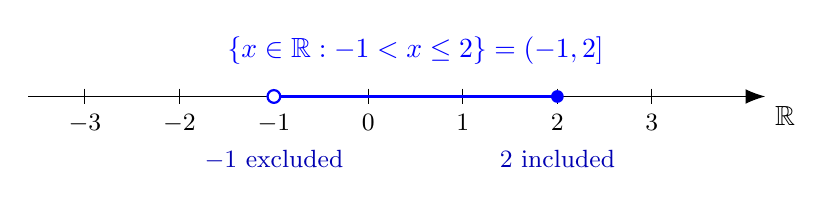
\begin{tikzpicture}[x=1.2cm]
	\draw[-{Latex[length=2.5mm]}] (-3.6,0) -- (4.2,0) node[below right] {$\mathbb{R}$};
	\foreach \x in {-3,-2,-1,0,1,2,3} {\draw (\x,0.1) -- (\x,-0.1); \node[below=3pt, font=\small] at (\x,0) {$\x$};}
	\draw[very thick, blue] (-1,0) -- (2,0);
	\draw[blue, thick, fill=white] (-1,0) circle (2.3pt);
	\fill[blue] (2,0) circle (2.3pt);
	\node[blue, above=8pt] at (0.5,0) {$\{x\in\mathbb{R}: -1<x\le 2\}=(-1,2]$};
	\node[blue!70!black, below=16pt, font=\small] at (-1,0) {$-1$ excluded};
	\node[blue!70!black, below=16pt, font=\small] at (2,0) {$2$ included};
\end{tikzpicture}
\end{document}
